\section{System design}
\label{sec:system_design}
~

No supervised learning model has been found in the literature to 
tackle the non-preemptive, global fixed-priority scheduling problem 
for single DAG tasks.
Therefore, we must first design a supervised learning model
that is able to approximate the computation of a priority-list for a single DAG task
that leads to the minimum makespan.

In order to have a supervised model, we need
to train the model on a set of already solved DAGs 
so that the model can learn how to approximate those solutions in a reasonable time.
Indeed, in supervised learning, the machine learning model 
predicts an output (forward pass) and then computes the error between
the predicted output and a known true output.
The gradient of the error function is then propagated through the network to tweak the model's 
trainable parameters, which is also called the backward pass (see Figure \ref{fig:supervised_learning}).
The issue with the supervised method is that we need to have true outputs,
that is priority lists that we know lead to the minimum makespan.
However, the problem is NP-hard which makes the computation
of those true labels expensive. The idea behind this supervised
method is to leverage the amount of training time with the performance
and scalability of the model, once it is trained.

\begin{figure}
    \centering
    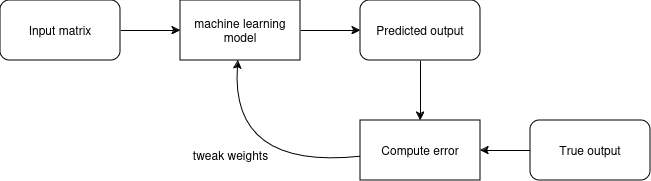
\includegraphics[width=\linewidth]{images/supervised_learning_diagram.drawio.png}
    \caption{The supervised learning method.}
    \label{fig:supervised_learning}
\end{figure}

\subsection{Supervised design}
~

\subsubsection{Input DAGs}
~

In machine learning, the input that we give to the model
needs to be in a matrix representation which the model can 
then process. Therefore, every DAG task needs to have
a matrix representation that encompasses the information 
required to make decisions about its execution priority order.  
Each input DAG  task will be represented using 
a matrix of numbers with each row being a node
and each column being a raw feature of a node.
The list of raw features is similar to what is proposed by \citet{Lee2021GlobalDagSchedDRL},
that is :
\begin{list}{}{}
    \item - the normalized wcet of the node, i.e., $C_i / L$ for node $i$ with $L$ being the total workload ;
    \item - the number of incoming neighbours ;
    \item - the number of outgoing neighbours ;
    \item - a boolean value of whether the node is the source or sink node ;
    \item - a boolean value of whether the node is part of the critical path of the DAG.
\end{list}

The wcet is widely used as a criteria for priority-list scheduling algorithm (RM, EDF\cite{buttazzo2005RMvsEDF}, etc.)
but it needs to be normalized to have the context information of the whole graph.
The number of incoming and outgoing neighbours makes it possible 
to take into account the inner structure of the graph to compute the execution order.
The source and sink nodes are particular nodes in that their priority
is not important because they will respectively execute first and last due to their dependency constraints.
Finally, the critical path plays a huge role in state-of-the-art heuristics\cite{He2019DagIntra}\cite{zhao2020DAGsched},
with nodes in the critical path often having higher priorities than those
that aren't.
An example of such a DAG task representation is shown in Figure \ref{fig:dag_task_matrix_example}.

\begin{figure}
    \centering
    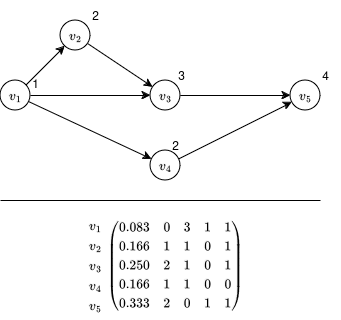
\includegraphics[width=\linewidth]{images/dag_matrix_example.drawio.png}
    \caption{Example dag task with 5 nodes a total workload of 12
    and the matrix representation of each node with the column respectively being the above list of features.}
    \label{fig:dag_task_matrix_example}
\end{figure}

\subsubsection{Output labels}
~
\label{sec:output_labels}
An Integer Linear Programming (ILP) solver will be used to compute
the optimal (minimum makespan) schedule for each DAG task and then
ordering the nodes according to their release time in the ILP schedule.

The output of the model will be a matrix of probabilities,
with each row being the index of a node and each column being the index of the priority.
There are as many priorities as there are nodes and 
the priority list of each DAG is then retrieved using the column
index of the maximum probability as the assigned probability, for each row.
Matrix output example for the DAG task shown in Figure \ref{fig:dag_task_matrix_example}
is shown in Figure \ref{fig:dag_output_matrix_example}.

\begin{figure}
    \centering
    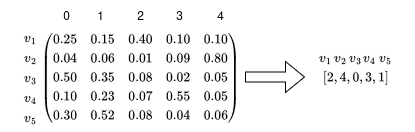
\includegraphics[width=\linewidth]{images/output_matrix_example.drawio.png}
    \caption{Example of an matrix output from the model, the predicted list of priorities (on the right)
    is retrieved from the probabilities.}
    \label{fig:dag_output_matrix_example}
\end{figure}

The ILP output matrix to compare the predicted output to is of the same shape
as the predicted output matrix with the probabilities being 1 on the optimal priority for each row 
, and 0 otherwise. For instance, if the optimal priority list for a DAG task of 3 nodes 
is [$\tau_1$: 0, $\tau_2$: 2, $\tau_3$: 1],
then the true label is the matrix :
$$
\begin{pmatrix}
    1 & 0 & 0\\
    0 & 0 & 1\\
    0 & 1 & 0
\end{pmatrix}
$$
With each row representing $\tau_1$, $\tau_2$ and $\tau_3$ respectively,
and the column represent the priorities 0, 1 and 2 respectively.
\subsubsection{Loss function}
~
\label{sec:loss_design}

The problem is being treated as a classification problem,
hence the binary cross-entropy loss function will be used.
This function is defined as follows :
\begin{equation}
    loss(x, y) = \sum_{i=1}^{n} -y_i\log(x_i)
\end{equation}
    
where $x$ is the flattened matrix representing the predicted output,
$y$ is the flattened matrix representing the true output (ILP output),
and $n$ is the number of element in $x$ and $y$.


\subsection{Model design}
~
\label{sec:model_design}

The model's architecture is very similar to the proposed encoder in \citet{Lee2021GlobalDagSchedDRL},
that is, the model is comprised of three modules.
Two feed forward networks and one attention-based graph convolutional network (see Figure \ref{fig:model_diagram}).

\begin{figure}
    \centering
    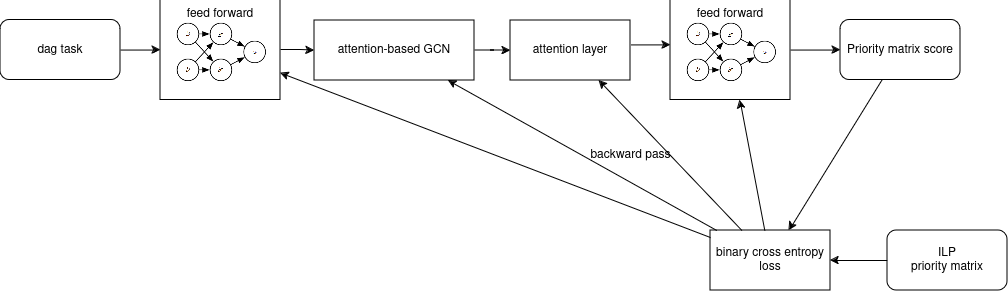
\includegraphics[width=\linewidth]{images/designed_model.png}
    \caption{The architecture diagram of the proposed supervised machine learning model.}
    \label{fig:model_diagram}
\end{figure}

\subsubsection{Feed forward networks}
~

The two feed forward networks have 3 layers with each 
layer $n$ producing the following output,
where $W_n \in \mathbb{R}^{5\times5}$ is the matrix of trainable weights
at layer $n$, $b_n \in \mathbb{R}^5$ is the bias and $X_n$ is either a node's vector representation
or the output of the previous layer, and $ReLU(x) = max(0, x)$:
\begin{equation}
    o_{n} = ReLU(W_{n}X_{n} + b_n),\, n \in \{1,2,3\}
\end{equation}
There is an exception for the second feed forward network where the last 
layer's output is computed using the following equation:
\begin{equation}
    o_{3} = \tanh(W_{3}X_{3} + b_3)
\end{equation}
where $W_3 \in \mathbb{R}^{nbPriorities \times 5}$,
$b_3 \in \mathbb{R}^{nbPriorities}$ and $\tanh$ is the 
hyperbolic tangent activation function.
Also, $nbPriorities$ corresponds to the number of different priorities
that can be assigned to each node.


\subsubsection{Graph Convolutional Network}
~

For each gcn layer, the input vector $X_k$ 
goes through an aggregation phase where,
given the set of incoming neighbours of node $v_i$, $\mathcal{N}_{in}(v_i)$, which includes
$v_i$, and the set of outgoing neighbours $\mathcal{N}_{out}(v_i)$, which also includes $v_i$,
the next vector representation $X_{k+1}$ is calculated by the following equation:

\begin{equation}
GCN(X) = AttentionModule(X, \mathcal{N}_{in}(v_i), \mathcal{N}_{out}(v_i))
\end{equation}

where $AttentionModule$ is defined by the Equations \ref{eq:attention_module}--\ref{eq:elu}:

\begin{multline}
    AttentionModule(X, \mathcal{N}_{in}(v_i), \mathcal{N}_{out}(v_i)) = \\
    ELU\left( W \left( Att(X, \mathcal{N}_{in}(v_i)) \oplus Att(X, \mathcal{N}_{out}(v_i)) \right) + b \right)
    \label{eq:attention_module}
\end{multline}

\begin{equation}
Att(X, \mathcal{N}(v_i)) = W\sum_{j \in \mathcal{N}(v_i)} \alpha_{ij} X_j
\label{eq:attention_submodule}
\end{equation}
Where 
\begin{equation}
    \alpha_{ij} = \frac{\exp \left ({ a ^{T} W X_{i} + b ^{T} W X_{j} }\right )}
    {{\sum _{k \in \mathcal {N}(v_{i})}} \exp \left ({ a ^{T} W X_{i} + b ^{T} W X_{k} }\right )}
\end{equation}

are the attention coefficients
which evaluates how important is $v_j$ to $v_i$'s vector 
representation, similar to what is done in \citet{Lee2021GlobalDagSchedDRL}.

Every $W$, $a$, and $b$ are different matrices of trainable parameters,
and $\text{ELU}$ is the exponential linear unit activation function (Equation \ref{eq:elu}).

\begin{figure}
    \centering
    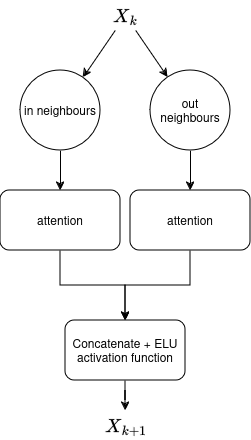
\includegraphics[width=0.5\linewidth]{images/gcn_update_aggregate_diagram.png}
    \caption{Diagram of the graph convolution network layer. $X_k$ is the transformed node vector representation
    and ELU is the exponential linear unit function (see Equation \ref{eq:elu}).}
    \label{fig:update_aggregate_diagram}
\end{figure}

\begin{equation}
\text{ELU}(x) = 
\begin{cases}
x, & \text{if } x > 0 \\
\exp(x) - 1, & \text{if } x \leq 0
\end{cases}
\label{eq:elu}
\end{equation}


The idea behind using attention is to make the model 
take into account the inner structure of the graph by 
looking at the importance of each node
compared to its neighbour nodes.
The GCN layer can be repeated several times 
to improve the model's capacity to better
capture the complexity of the graph structure.
Unfortunately, when testing with 3 GCN layers,
we ran into an oversmoothing problem\cite{chen2020oversmoothing}, which lead us 
to restrict the number of GCN layers to just one layer.

\subsection{Computing the labels}
~

\subsubsection{Computing the optimal schedule}

\citet{yip2023letsynchronise} proposed an ILP-based
scheduling solver for event-chains of time-triggered tasks
using the Logical Execution Time paradigm\cite{kirsch2012logical}.
Their work aimed at minimizing the sum of dependency delays 
between the job instances of each task and they have recently added
support for multicore architectures\footnote{https://github.com/mkuo005/LET-LP-Scheduler}.

Although their minimizing problem is slightly different from ours, 
we can convert our minimizing problem and then use their LET solver by converting each DAG task 
to an event-chain of LET task.
To do this, each node needs to be converted to an LET task which 
implies adding an initial offset, activation offset, LET interval duration and a period
to every node.
Hence, for each node, the initial offset and activation offset will
be set to 0 and the LET interval duration will be set to the node's wcet.
For the period, every node in a DAG will have the same period which will
be equal to the total workload squared.
The wcet of a node will be the wcet of its LET task version.
Lastly, each path in the DAG will represent an even-chain of tasks.

Unfortunately, minimzing the sum of dependency delays (i.e., Equation 6 in \citet{yip2023letsynchronise}) is not equivalent
to minimizing the makespan of a DAG (see Figure \ref{fig:counter_example_minsumdep})
but we can change the objective function to the end execution time
of the sink node, i.e., the node which doesn't have any successors,
which is the definition of the makespan.
This effectively makes the solver minimize the makespan of DAG task
which is precisely the problem at stakes.
The other modifications involve setting the configuration parameters $useOffset$,
$useHeterogeneousCores$ and $restrictTaskInstancesToSameCore$ to
$False$\footnote{See the github repository for more details \url{https://github.com/FelicienFG/research-project-AUT/}.}.

\begin{figure}
    \centering
    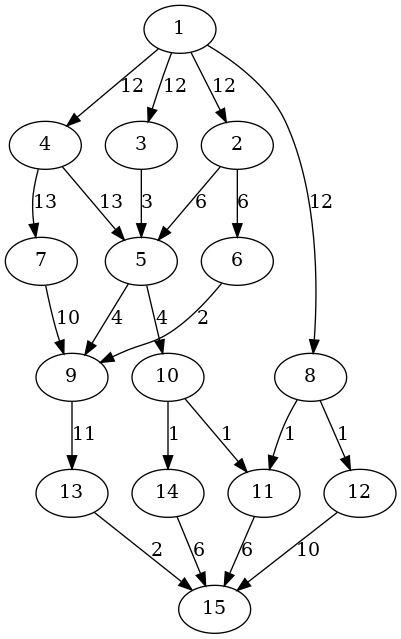
\includegraphics[width=0.5\linewidth]{images/Tau_108.png}
    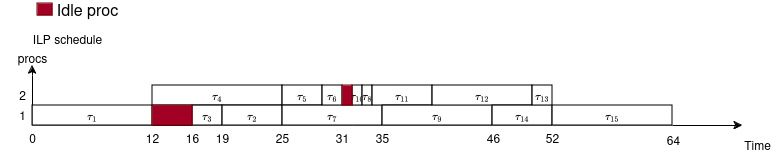
\includegraphics[width=\linewidth, height=70px]{images/schedule_ilp_fail_correct.png}
    \par Schedule a)
    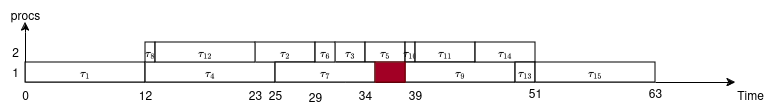
\includegraphics[width=\linewidth, height=55px]{images/schedule_example_ilpfail_better.png}
    \par Schedule b)
    \caption{Example of a DAG task (top image) where the schedule that the ILP solver outputs (the schedule a))
    produces a longer makespan (64) but smaller sum of dependencies delays (400) than 
    the schedule b) with a makespan of 63 and a sum of dependencies delays of 427.}
    \label{fig:counter_example_minsumdep}
\end{figure}

\subsubsection{Computing the optimal priority-list}
~

Once the optimal schedule (i.e., the schedule yielding the minimum makespan)
is computed,
the optimal priority-list can be obtained from the schedule 
by looking at the start times of each node and increasing the priority 
according to the node's start time.
The sooner the start time, the higher the priority.

For instance, for the non-optimal schedule shown in Figure \ref{fig:counter_example_minsumdep} (schedule a)),
the corresponding priority-list would be 0 for node $\tau_1$, 1 for node $\tau_4$,
etc, i.e., [$\tau_1$: 0, $\tau_2$: 3, $\tau_3$: 2, $\tau_4$: 1, $\tau_5$: 4, $\tau_6$: 6, $\tau_7$: 5, $\tau_8$: 8,
 $\tau_9$: 10, $\tau_10$: 7, $\tau_11$: 9, $\tau_12$: 11, $\tau_13$: 13, $\tau_14$: 12, $\tau_15$: 14].
This priority list is then converted to a matrix by the process described
at the end of Section \ref{sec:output_labels}.

\subsection{Makespan calculation}
~

The main performance metric that will be used in the evaluation
is the makespan, i.e., the end execution time of the sink node of a DAG.
The exact computation of the makespan is done by simulating a 
simple non-preemptive global fixed-priority scheduler, for which the algorithm
is described in the Figure \ref{fig:algo_makespan}.
The basic idea is to have a ready queue that contains the nodes
that have their precedence constraints met
and the nodes still waiting to have their dependencies met 
are in the waiting list. Each loop iteration, the waiting list and ready queue
are updated and the first idle processor gets the node at the top of 
the ready priority queue (see Figure \ref{fig:algo_makespan} and \ref{fig:algo_makespan_details}).

\begin{figure}
    \centering
    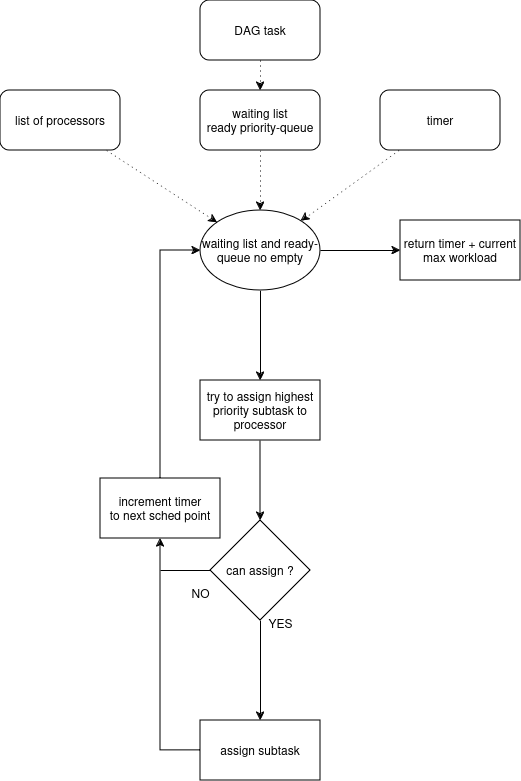
\includegraphics[width=\linewidth]{images/makespan_computation_algorithm_global.png}
    \caption{Top view of the makespan computation algorithm.}
    \label{fig:algo_makespan}
\end{figure}

\begin{figure}
    \centering
    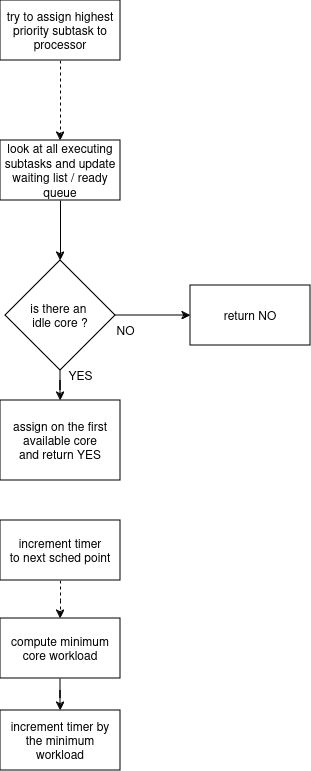
\includegraphics[width=0.8\linewidth]{images/makespan_computation_algorithm_assign.png}
    \caption{Algorithms for assigning the highest priority node (or subtask) to a processor (top)
    and for incrementing the timer to the next scheduling point (bottom).}
    \label{fig:algo_makespan_details}
\end{figure}

The implementation will be done in C++ with bindings to python to make
the makespan computation faster.

% config for 20,30 nodes : 
%  "dag_config": {
%    "parallelism": 8,
%    "layer_num_min": 5,
%    "layer_num_max": 8,
% config for 10 nodes :
%"dag_config": {
%    "parallelism": 8,
%    "layer_num_min": 3,
%    "layer_num_max": 8,
% config for 40 nodes :
%"dag_config": {
%    "parallelism": 8,
%    "layer_num_min": 7,
%    "layer_num_max": 10,
% config for 50 nodes :
%"dag_config": {
%    "parallelism": 8,
%    "layer_num_min": 10,
%    "layer_num_max": 15,
%config for varying number of parallelism (n=30nodes)
%"dag_config": {
%    "parallelism": [4-6, 7],
%    "layer_num_min": 8, (5 for p = 7)
%    "layer_num_max": 13, (10 for p = 7)